\section{Diagnostic Methods Supplemental Information}

\subsection{Microwave Scattering}
Erevant, formerly Sage MM

SOM-90305213-10-S1
90 GHz, ±0.25 GHz Tuning Bandwidth, +13 dBm Output Power, WR-10 Waveguide, W-Band Mechanically Tuned Gunn Oscillator

SBP-7531141015-1010-E1
75 to 110 GHz, 10 dB Gain, +15 dBm P1dB, In-line WR-10 Waveguide, W-Band Power Amplifier

SWP-90310404-10-E1
90 to 105 GHz, 20 dB Port Isolation, WR-10 Waveguide, W-Band, 4-Way In-line Power Divider

STP-18-10-M2
W-Band Phase Shifter
75 to 110 GHz, 0 to 180° Range, WR-10 Waveguide

SFQ-75311415-1010SF-N1-M
Quadrature Mixer or Phase Detector W Band
LO and RF Frequency: 75 to 108 GHz
IF Frequency: DC to 20 GHz (Typ) 
LO Pumping Level: +15 dBm (Typ) 
Conversion Loss: 15 dB (Typ) 
I/Q Phase Error: +/-15 Degrees (Typ) 
RF & LO Connectors: WR-10 Waveguide with Anti-Cocking 
UG-387/U-M
IF Connectors: SMA(F) 
Outline:FQ-W1M-A
ECCN:EAR99
Schedule B/HTS Code:8542390000

\begin{figure}[]
\centering
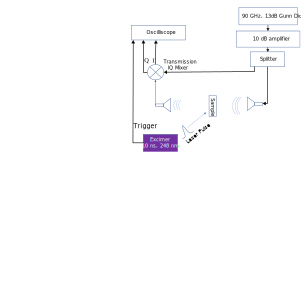
\includegraphics[width=0.8\textwidth]{\repodir/final/figures/SI/output/MWS_Setup_Silicon.png}
\caption{Microwave scattering setup for silicon wafers.}
\label{fig:SI_MWS_Setup_Silicon}
\end{figure}

\begin{figure}[]
\centering
\includegraphics[width=0.8\textwidth]{\repodir/final/dataset/output/figures/mws_nothing_T0.png}
\caption{A) Measurement of transmission without any torch, B) position dependent transmission measurement.}
\label{fig:SI_MWS}
\end{figure}

\ref{fig:SI_mws_processing_overview} shows the processing steps for the MWS data. 



\begin{figure}[]
\centering
\includegraphics[width=0.8\textwidth]{\repodir/experiment/analysis/mws/output/figures/mws_processing_overview.png}
\caption{Microwave processing overview}
\label{fig:SI_mws_processing_overview}
\end{figure}


\subsection{Laser Profile}


\begin{figure}[]
\centering
\includegraphics[width=0.8\textwidth]{\repodir/experiment/analysis/mws/output/figures/laser_profile.png}
\caption{Laser profile measurement}
\label{fig:SI_Laser_Profile}
\end{figure}